\documentclass[10pt,letter]{article}
	% basic article document class
	% use percent signs to make comments to yourself -- they will not show up.

\usepackage{url}
\usepackage{amsmath}
\usepackage{amssymb}
\usepackage[makeroom]{cancel}
	% packages that allow mathematical formatting

\usepackage{graphicx}
	% package that allows you to include graphics

\setlength\parindent{0pt}

\usepackage{pdfpages}

\usepackage{setspace}
	% package that allows you to change spacing


\let\emptyset\varnothing

\usepackage{enumerate}


\usepackage{siunitx}
\sisetup{mode=text,range-phrase = {\text{~to~}}}

\onehalfspacing
	% text become 1.5 spaced

\usepackage{fullpage}
	% package that specifies normal margins

\usepackage{datetime}

\usepackage{tikz}
\usetikzlibrary{arrows}
\usetikzlibrary{positioning}


\begin{document}
	% line of code telling latex that your document is beginning


\title{CPSC 458 Final Project Write Up \\ \url{http://cpsc458-brooks.herokuapp.com}}
\date{\today}

\author{Jason Brooks}

\maketitle 
	% tells latex to follow your header (e.g., title, author) commands.

For the final project, I decided to implement the default project option: constructing a recommendation engine for computers. I constructed a sleek user interface over the recommendation pipeline that allows users to input what they're looking for in a computer, and receive a tailored recommendation based on their preferences and prior computer history. Below is an overview of how the application works, and how it was created. The site can be tried at \url{http://cpsc458-brooks.herokuapp.com}.

 \begin{figure}[htbp]
    \centering
    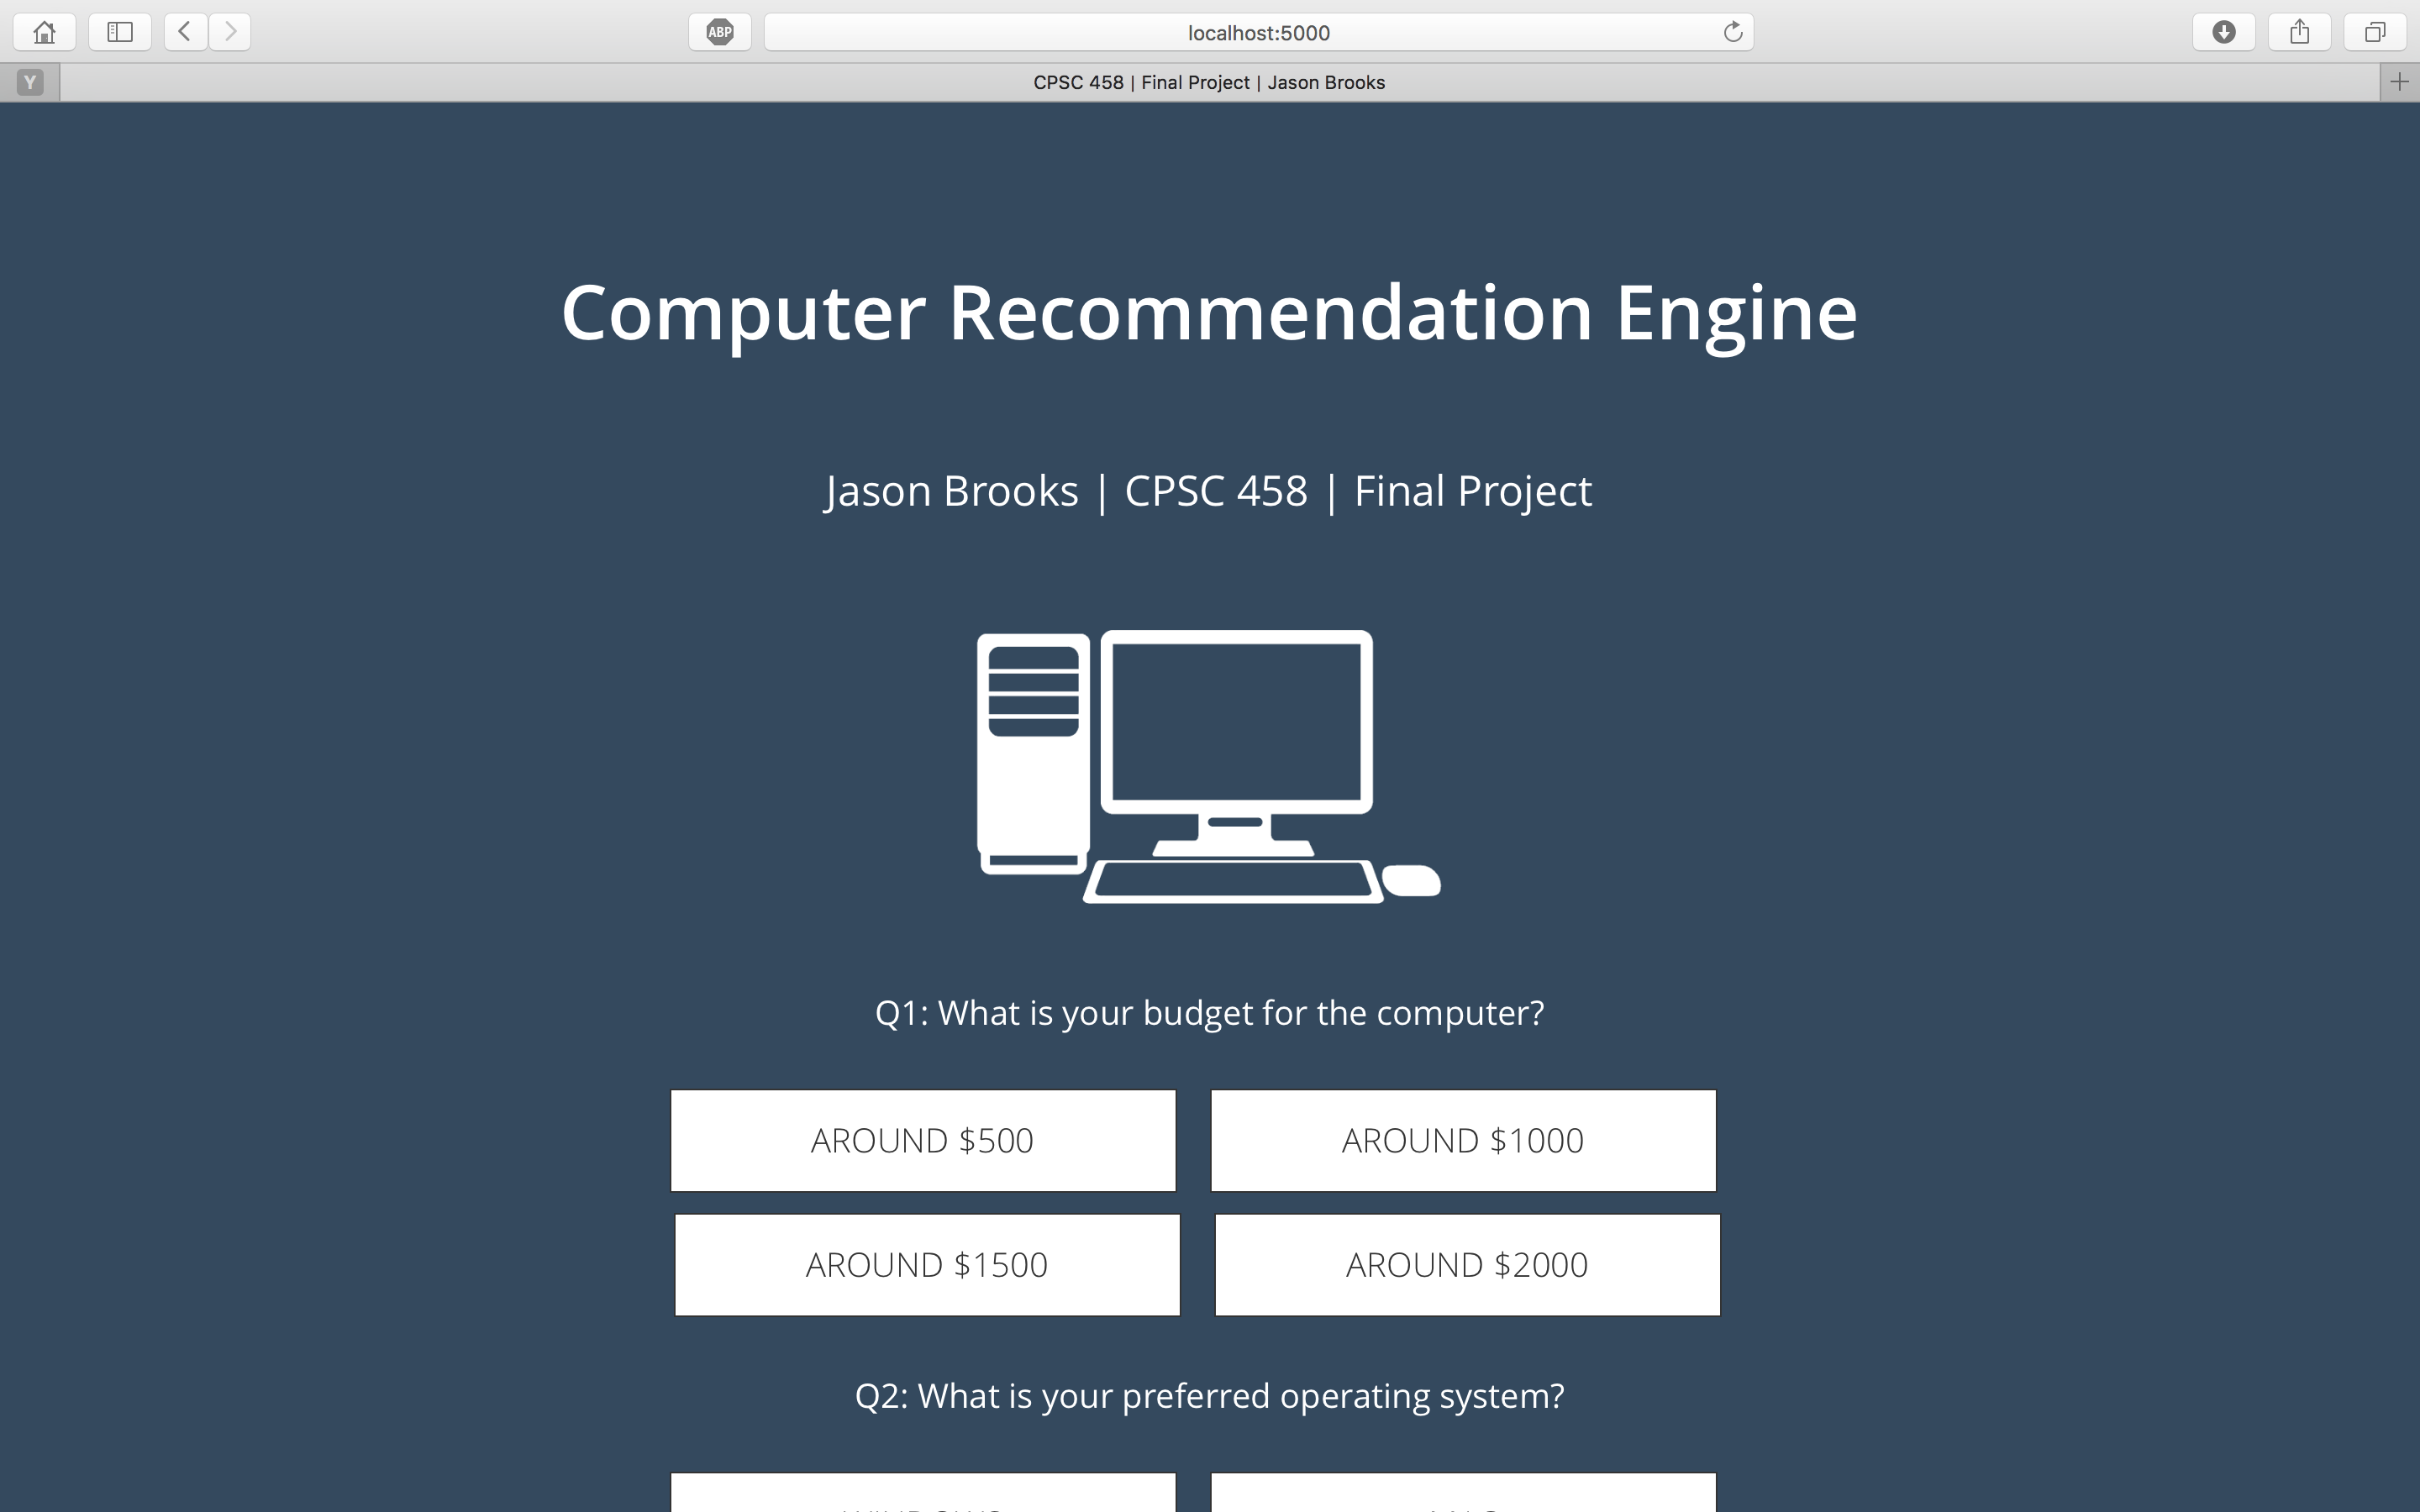
\includegraphics[width=7.0in]{homepage.png}
\end{figure}

\section{Scope of the Project}
This project is comprised of many different parts, all integrated under one central Flask web application, with a SQL database. The Flask app employees three main sections - the code for populating the data set, the code for making the recommendation, and the machine learning code for training the model over time. Below is an overview of each part.

\subsection{Populating the Dataset}

While conducting research for the project, I came across the website \url{http://www.lappylist.com}, which provides information about popular computer models, including hardware and software specifications for each. To provide some realistic models to test the effectiveness of my recommendation engine, I created a crawler to pull and normalize the data about each computer. The file \texttt{computerModelCrawler.py} under the main directory provides the code for crawling the contents of all computers listed on their site. The result of this script is a list of lists, with each sublist containing information about a particular computer model. All in all, this yielded 109 unique computers with complete specifications.\\

The data from the crawler was error prone and non-clean. To populate my database with computer models, I created a script to reset the database called \texttt{reset.py} under the main directory. After examining with the raw data, I was able to program the reset script to sanitize each field that I cared about. These fields are analogous to the questions asked in the user survey about their computer preferences. Specifically, I sanitized and normalized data about the computers operating system, battery life, hard drive space, price, and screen size. To deliver accurate information and specifications about the computer when the recommendation is eventually made, I also store the raw data in separate columns of my database.

\subsection{Recommendation Code}

The next major part of the project was the actual recommendation algorithm. As mentioned, I asked six questions regarding computer preferences in the user survey. I decided to use a weight-based system, where each of these preferences was assigned an initial weight. I had all the weights sum to 1.0, where budget and operating system were each assigned a weight of 0.3, with the other parameters each assigned a weight of 0.1. After playing with and testing the recommendation algorithm, it seemed that operating system and budget are two parameters that people are much more strict about in terms of preferences and needs, as compared to parameters like hard drive space and RAM, which most people are not as technologically savvy about.\\

One of the main features of the recommendation engine is a set of functions, one for each feature in the questionnaire, that compute a score as a function of the target specification for a particular feature (what the user requests) and the feature of a given computer model. The scoring system works like golf -- the closer the score to 0, the better a match. If the user answers the survey question by saying a given feature does not matter to them, then the feature is also assigned a score of 0. Similarly, if the specification of a given computer model is greater than the target, we also assign a score of 0 since this means the specification excels over what the user is looking for. If a given computer model has a specification lower then the target, then the score is a positive value, representing that the feature is not in line with what the user is looking for.\\

So with the initial weights set, the first step in the process is to adjust the weights for each parameter based on the previous computer models that the person owned (see \texttt{splash/\_\_init\_\_.py}). I specifically ask for a separation of computer models that the person liked and disliked. Then, the function \texttt{update\_weights} (in that same file) cycles through each computer on the like/dislike list and adjusts the weights accordingly. We subtract from the weights for computers that the person liked, and add to the weights for computers that the person disliked.\\

After getting adjusted weights, the recommendation engine computes a score for each laptop in the database, where (once again) the lowest score is the best computer. Each of the scoring functions for each feature is run on each computer in the database, and the final score for that computer is the summation of the scores from each feature's function. In this process, weights are adjusted, such that if a person has no preference for a given feature, it's weight is assigned to 0, and the weights for all other functions are once again normalized so that they sum to 1.0.\\

Finally, the top three recommendations are displayed in real time on the Web site. The engine looks at the weights and computer that is ultimately recommended to build the text that explains why the given model was presented to the user.

 \begin{figure}[htbp]
    \centering
    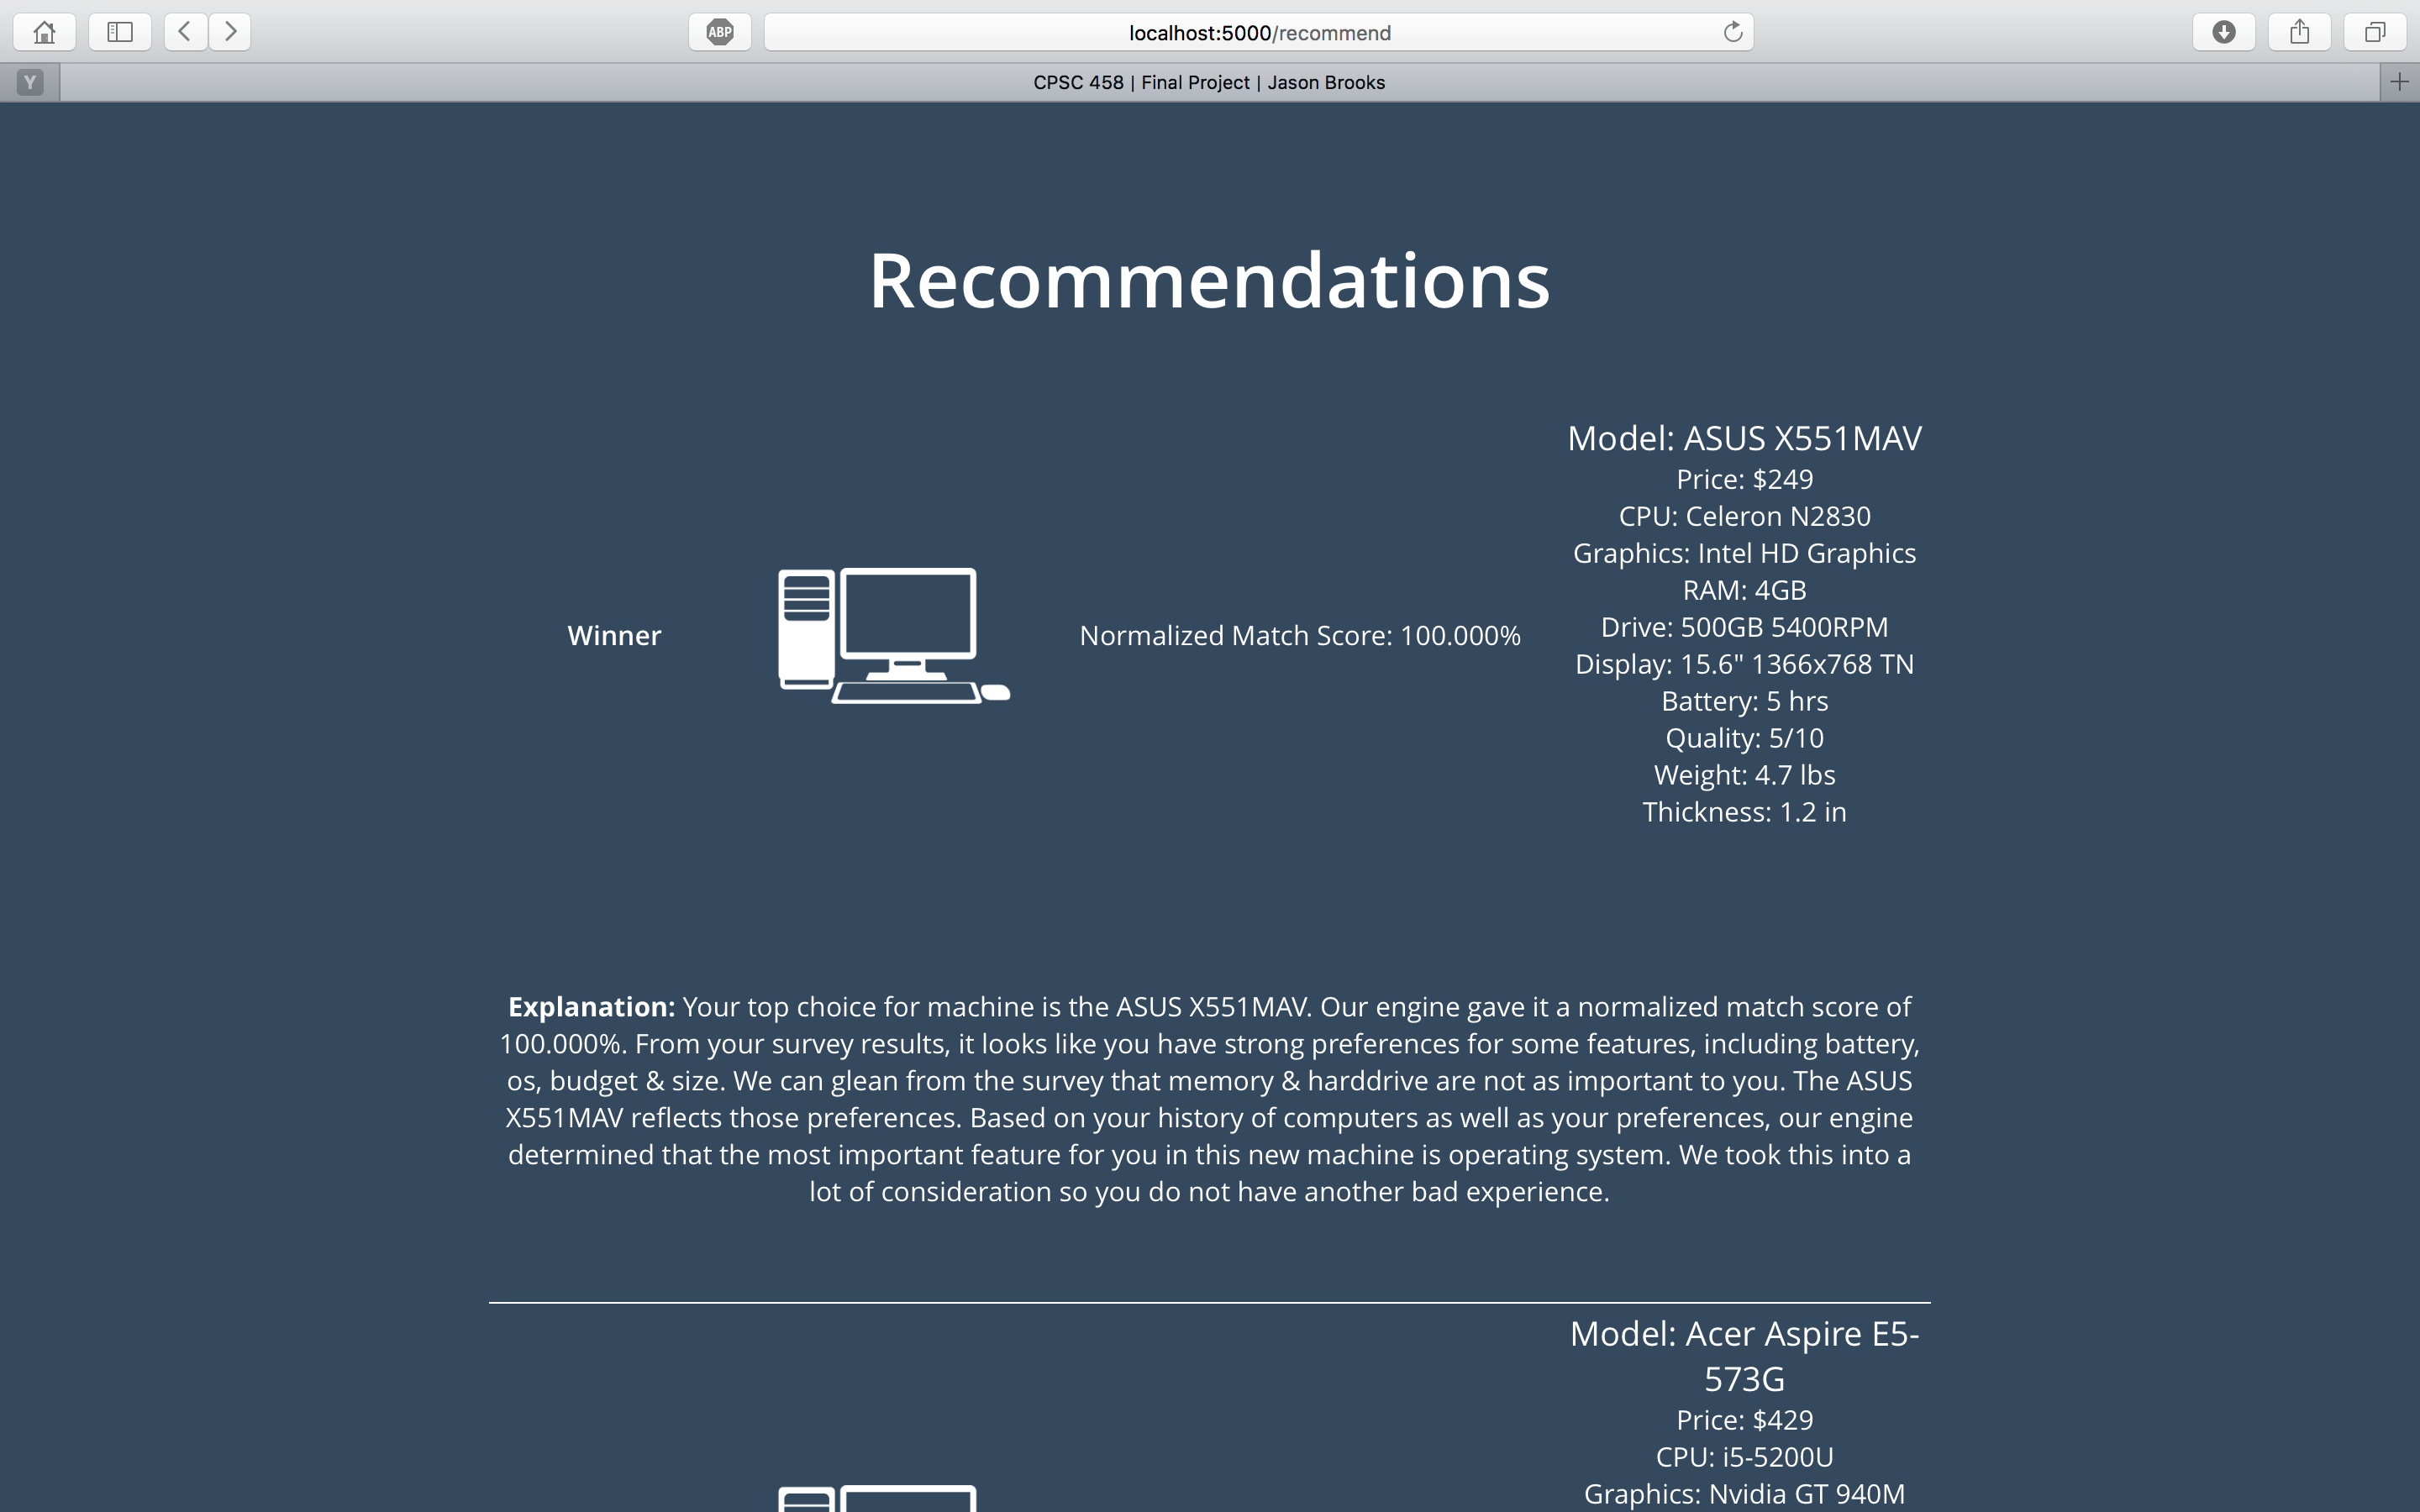
\includegraphics[width=7.0in]{recommend.png}
\end{figure}

\subsection{Machine Learning}

My computer recommendation engine employs a very basic version of machine learning. Basically, the database maintains the weights that are generated for each user, and computes new starting weights on each successive iteration. The purpose of this is to learn what people like over time. If the engine realizes that a lot of people value a specific criteria for their recommendations, then the weights should be updated to reflect that to give more accurate predictions in the future.

\end{document}
	
	
	
	
	
	
	
	
	
	
	
	